% Name: Cofactor expansion
% Description: Striking out row 1 and column 2 of A leaves the minor M₁₂, and the determinant expands along the first row as a sum of entries times cofactors.
% Tags: determinant, cofactor, minor, Laplace expansion

\usepackage{amsmath}
\usetikzlibrary{matrix, positioning, calc}

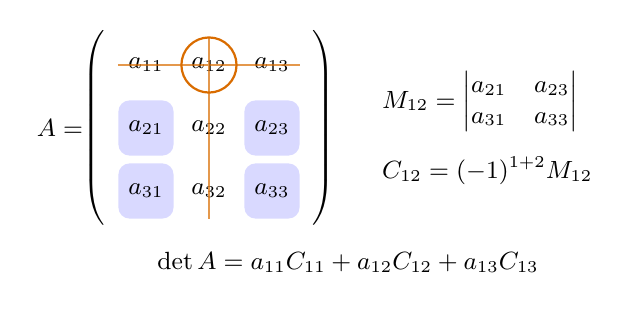
\begin{tikzpicture}[every node/.style={font=\small}]
  \matrix (m) [matrix of math nodes, left delimiter=(, right delimiter=), nodes={minimum size=7mm}, column sep=1mm, row sep=1mm] {
    a_{11} & a_{12} & a_{13} \\
    a_{21} & a_{22} & a_{23} \\
    a_{31} & a_{32} & a_{33} \\
  };
  \node[left=2mm of m] {$A =$};
  \node[draw=orange!85!black, thick, circle, inner sep=0pt, minimum size=7mm] at (m-1-2) {};
  \draw[orange!85!black, thick, opacity=0.7] (m-1-1.west) -- (m-1-3.east) (m-1-2.north) -- (m-3-2.south);
  \foreach \r/\c in {2/1, 2/3, 3/1, 3/3} \node[fill=blue!15, rounded corners, minimum size=7mm, inner sep=0pt] at (m-\r-\c) {$a_{\r\c}$};
  \node[right=8mm of m, align=left] (minor) {$M_{12} = \begin{vmatrix} a_{21} & a_{23} \\ a_{31} & a_{33} \end{vmatrix}$ \\[8pt] $C_{12} = (-1)^{1+2} M_{12}$};
  \node[below=4mm] at ($(m.south)!0.5!(minor.south)$) {$\det A = a_{11} C_{11} + a_{12} C_{12} + a_{13} C_{13}$};
\end{tikzpicture}
